\documentclass[document.tex]{subfiles}
\begin{document}

\chapter{Feature Reduction and Classification}
\noindent Feature mining generally refers to transform a high dimensional correlated dataset into a low dimensional uncorrelated data space. It can be done by following two steps:
\begin{itemize}
	\item Feature extraction
	\item Feature selection
\end{itemize}

\section{Feature Extraction}
\noindent Principal component analysis (PCA)\cite{7} is one of the most popular unsupervised feature extraction technique.The principal component analysis is based on the fact that neighboring bands of hyperspectral images are highly correlated and often convey almost the same information about the object. The PCA employs the statistic properties of
hyperspectral bands to examine band dependency or correlation. This transformation
is based on the mathematical principle known as eigenvalue decomposition of the
covariance matrix of the hyperspectral image bands to be analyzed. The new transformed uncorrelated variables called principal components (PCs). First few variable contains most of the variation of the original data. If a hyperspectral image form M = i * j * k dataset where i is number of rows, j is number of columns and k is the number of bands of the dataset. Then after applying PCA to our dataset, we can use a small portion of k and still find almost all variations of our data. $X_1,X_2,X_3,....,X_n$ is the bands of the dataset. 
\begin{comment}
\begin{figure}[H]
	\begin{center}
		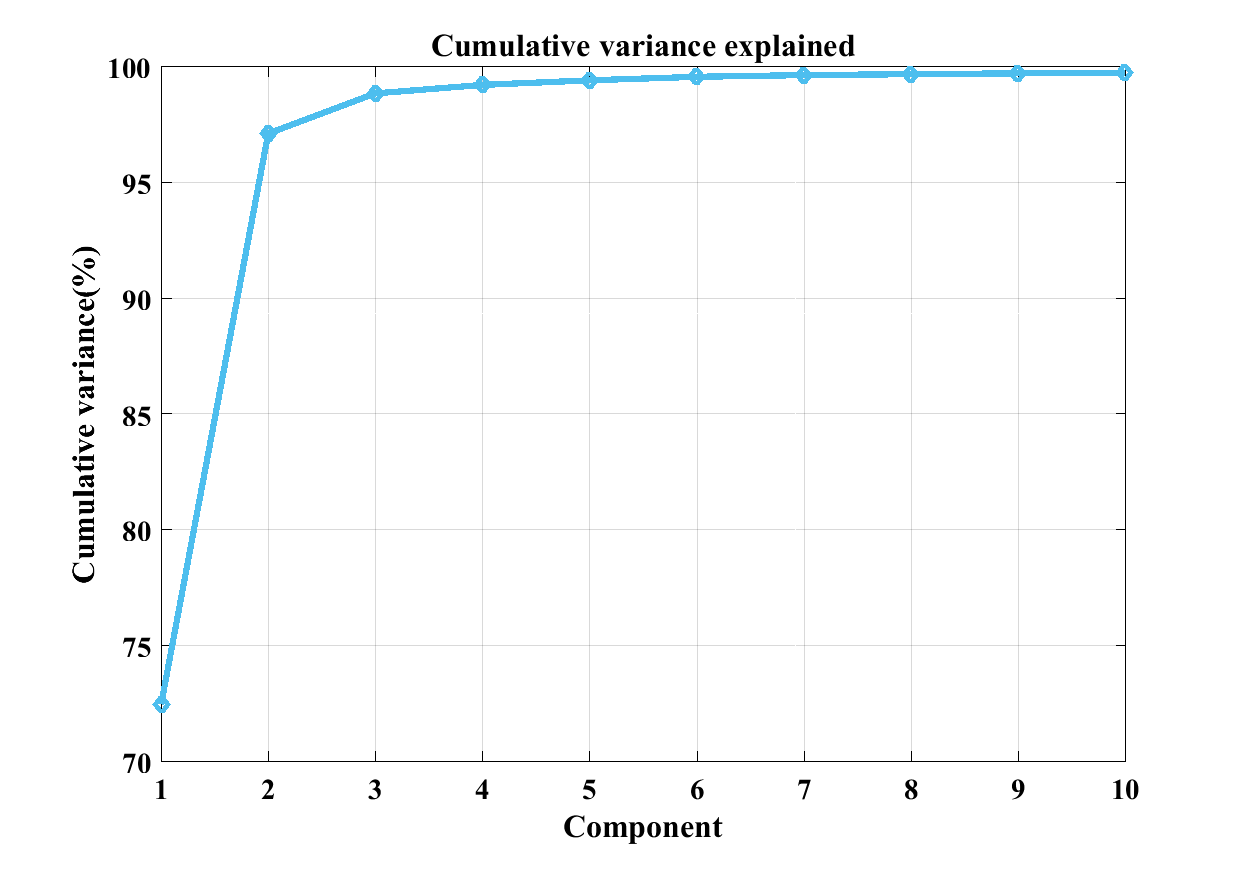
\includegraphics[height=8.0cm]{imgs/variance.png}
	\end{center}
	\caption{Cumulative variance of bands obtained via PCA}
	\label{fig:Cumulative variance of bands obtained via PCA}
\end{figure}
\end{comment}
\noindent For calculating PCA we first subtract mean form the dataset. The mean is calculated as
\begin{equation}
\overline{X} = \dfrac{\sum_{i=1}^{n} X_i}{n}
\label{eq:Mean}
\end{equation}
The covariance matrix between any two dimension can be calculated as:
\begin{equation}
COV(X,Y) = \dfrac{\sum_{i=1}^{n}(X_i - \overline{X})(Y_i - \overline{Y})}{n-1}
\end{equation}
Covariance matrix is a square matrix. Eigenvalue and eigenvector is calculated from covariance matrix. Eigenvector that has the highest eigenvalue is the first principal component. Arrangement of eigenvectors according to descending order of eigenvalues creates a matrix of new set of data whose first few column can be chosen for further use.
 
\section{Feature Selection Based on Normalized Mutual Information}
\noindent Mutual Information (MI) measures the amount of information one random variable holds about the other random variable\cite{20} by quantifying dependencies of those variables. Mutual information of two random varibles X and Y can be defined as:
\begin{equation}
I(X,Y) = \sum_{y=1}^{L1}\sum_{x=1}^{L2}p(x,y)\log\dfrac{p(x,y)}{p(x)p(y)}
\end{equation}
where x, y are the pixel values and L1, L2 are the maximum
pixel values of the input images. P(x,y) is joint probability distribution function and P(x) and P(y) is marginal probability distribution function of variable X and Y respectively. If two variable x and
y are independent, x does not know any information about y and vice versa. So their
mutual information will be zero. According to Shannon’s information theory, if the
probability of a random variable x is P(x) then uncertainty of x measured by entropy\cite{20} is:
\begin{equation}
H(x) = -p(x)log(p(x))
\end{equation}
Here mutual information can also be described as:
\begin{equation}
I(X,Y) = H(X) + H(Y) - H(X,Y)
\end{equation}
Where H(A) and H(B) are the entropies of A and B and H(A,B)
is their joint entropy. Now by calculating mutual information between class label $c = c_1,c_2,....c_N$ and bands $f = f_1,f_2,...f_N$ of the hyperspectral image we can select relevant features for classification. Each feature will be selected in descending order $I_1 \geq I_2 \geq I_3 \geq....\geq I_N$. Feature with highest mutual information contains most information. It is difficult to use the value given by (4.3) directly in an absolute sense, as it is affected by the entropy of the two variables and not bounded to [0, 1]. A few methods to normalize mutual information are available to give a new value between 0 and 1, where 0 is the value for the independent case and 1 for the identical or one-to-one relationship case. Normalized mutual information (nMI)\cite{21} is defined as follows:
\begin{equation}
\hat{I}(X,Y) = \dfrac{I(X,Y)}{\sqrt{I(X,X)}\sqrt{I(Y,Y)}}
\end{equation}

\subsection{Original Dataset Plus nMI Approach}
\noindent In feature selection, the relevant features have important
information required to produce the classification output. The aim of feature selection is to find only informative features $k < n$ for a dataset. If the reference image is f and original dataset is x then the normalized mutual information between f and x is given below:
\begin{equation}
\hat{I}(x_i,f_j) = \dfrac{\sum_{i}\sum_{j} p(x_i,f_j)\log\dfrac{p(x_i,f_j)}{p(x_i)p(f_j)}}{\sqrt{I(x_i,x_i)}\sqrt{I(f_j,f_j)}}
\end{equation}  

\subsection{PCA Dataset Plus nMI Approach}
\noindent In order to find informative features from the transformed features
obtained by unsupervised feature extraction technique principal component analysis (PCA) normalized mutual information (nMI) is applied as below. If the reference image is f and PCA transformed dataset is y then the normalized mutual information between f and y is given below:
\begin{equation}
\hat{I}(y_i,f_j) = \dfrac{\sum_{i}\sum_{j} p(y_i,f_j)\log\dfrac{p(y_i,f_j)}{p(y_i)p(f_j)}}{\sqrt{I(y_i,y_i)}\sqrt{I(f_j,f_j)}}
\end{equation}  

\section{Proposed Feature Reduction Method}
\noindent The proposed method is a target class oriented feature selection technique which select relevant features for each class of the dataset using principal component analysis (PCA) as feature extraction\cite{7} and normalized mutual information (nMI) as features selection\cite{9}. At first, the unsupervised feature extraction technique PCA is applied to find uncorrelated dataset in smaller data space. Then normalized mutual information (nMI) with two constraints to maximize general relevance and minimize redundancy on the components obtained via PCA is applied for feature selection\cite{21}. Here we consider one class of the dataset at a time and make all others as the background class. For each class of the dataset feature selection method is applied to obtain a relevant feature space to classify that class. Finally kernel support vector machine (SVM) is applied for classification purpose of the data set\cite{11}. Here first SVM use those selected features of each class to train a model for that specific class and test data to find test result for that specific class. RBF kernel\cite{22} is used in SVM as the relationship between class label C and datase $X_i$ is nonlinear. K-fold cross validation is applied to find correct parameter C and $\gamma$ of KSVM for each target class of the dataset. Finally average of those accuracy for each class is the final classification accuracy.

\section{Experimental Procedure}

\subsection{Feature Extraction}
\begin{itemize}
	\item \textbf{Step 1: Get input data. }\\
	For processing hyperspectral image I have converted 3 dimensional data cube into 2 dimensional spaces which I will use
	as input data for PCA.\\
	Input data = [Band1 image,band2 image, . . . . . . . .,Band 220 image]
	\item \textbf{Step 2: Calculating the mean of each image band and then subtracting
		the mean from the original.}\\
	Calculating the mean across each dimension and then subtracting along the dimensions. This produce images with mean value of 0. This mean subtracted data is
	represented by adjusted data.\\ Adjusted data = [Band1 image-mean1, band2 image-mean2 , . . . .,Band220 image-mean220]
	\item \textbf{Step 3: Calculating the covariance of the mean subtracted image.} \\
	In the 3rd step, I have calculated the covariance of the data got from step 2. From
	the non-diagonal value of the covariance matrix I got the information about how
	the dimensions of data are related to each other.
	\item \textbf{Step 4: Calculating the eigenvector and eigen values of the covariance matrix.} \\
	From the covariance matrix I have calculated the eigenvectors and eigen values
	matrix. This eigenvectors information is very important as they provide information
	about the characteristics of input data. Eigen values indicate the variance and
	eigenvectors indicate to which direction. For 220 dimensions I have got 220 eigen
	values and 220 eigen vectors. Among the 220 vectors one provides a best fitting of
	the input data.
	\item \textbf{Step 5: Forming feature vector by choosing the significant component.}\\
	The eigen vectors are rearranged according to the higher value of the eigen values.
	The eigenvector with the highest eigen value is the principal component of the
	data set and it has the largest relationship with the input data and dimension.
	This component contains the maximum feature of the input patterns. A subset of
	the eigenvectors with significant eigen values collected from all the eigenvectors is
	called feature vector.
	\item \textbf{ Step 6: Calculating the reduced data set and getting back the original
	data.}\\
	This is the final step of principal component analysis. From the chosen components
	defined as feature vectors I have got the data set with reduced dimensionality from
	the following equation.\\
	Final data (reduced in dimensionality) = Feature vector $\times$ Adjusted dataset\\
	Where, the adjusted dataset means dataset with mean value of 0. The original data
	is obtained by the following equation. Data obtained from the following equation
	will be slightly different from the original input data as some of the noise of the
	input data is removed by PCA when subset of the Eigen vectors are used. Original
	Dataset = ($Featurevector^T$ $\times$ Final data) + mean of each band image.
\end{itemize}

\subsection{nMI Based Feature Selection}
\begin{itemize}
	\item \textbf{Step 1: Normalizing dataset into a range}\\
	In my analysis I have normalized the dataset in 1 to 64 range. Then calculated a 64 $\times$ 64 probability table from which I have calculated the marginal probability and the joint probability of variable(s). 
	\item \textbf{Step 2: Calculating mutual information between class labels and bands}\\
	To select or rank best features for classification of the dataset I have calculated mutual information according to equation (4.3) between class labels and each band of the dataset.
	\item \textbf{Step 3: Calculating normalized mutual information}\\
	To normalize mutual information values between 0 to 1 I have used equation (4.6). Then I have used this normalized mutual information values to select effective features for the classification of the dataset. 
\end{itemize}
\subsubsection{Original Dataset Plus nMI Approach}
\begin{itemize}
	\item \textbf{Step 1: Get input data}\\
	In this analysis I have used original hyperspectral data set. I have taken all 220 bands into consideration. Then I generate class labels of the sample. I have taken
	fourteen classes which label 1 To 14.
	\item \textbf{Step 2: Normalizing dataset into a range}\\
	I have normalized the dataset in 1 to 64 range. Then calculated a 64 $\times$ 64 probability table from which I have calculated the marginal probability and the joint probability of variable(s). 
	\item \textbf{Step 3: Calculating mutual information between class labels and bands}\\
	To select or rank best features for classification of the dataset I have calculated mutual information according to equation (4.3) between class labels and each band of the dataset.
	\item \textbf{Step 4: Calculating normalized mutual information}\\
	To normalize mutual information values between 0 to 1 I have used equation (4.6). Then I have used this normalized mutual information values to select effective features for the classification of the dataset. 
\end{itemize}
\subsubsection{PCA Dataset Plus nMI Approach}
\begin{itemize}
	\item \textbf{Step 1: Get input data}\\
	In this analysis I have used dataset obtained via principal component analysis. I have taken first 20 principal components into consideration. Then I generate class labels of the sample. I have taken
	fourteen classes which label 1 To 14.
	\item \textbf{Step 2: Normalizing dataset into a range}\\
	I have normalized the dataset in 1 to 64 range. Then calculated a 64 $\times$ 64 probability table from which I have calculated the marginal probability and the joint probability of variable(s). 
	\item \textbf{Step 3: Calculating mutual information between class labels and bands}\\
	To select or rank best features for classification of the dataset I have calculated mutual information according to equation (4.3) between class labels and each band of the dataset.
	\item \textbf{Step 4: Calculating normalized mutual information}\\
	To normalize mutual information values between 0 to 1 I have used equation (4.6). Then I have used this normalized mutual information values to select effective features for the classification of the dataset. 
\end{itemize}
\subsection{Proposed method}
The algorithm of the proposed feature reduction method can be
summarized as follows:
\begin{itemize}
	\item \textbf{Step 1:} Perform PCA on the original image. Extract the feature of the PCA image, i.e, select the high variance bands.
	\item \textbf{Step 2:} Extract the training data and training label from the
	selected features.
	\item \textbf{Step 3:} Extract a target class at a time from the dataset, i.e, make a class as foreground and all other class as background. 
	\item \textbf{Step 4:} Apply NMI between the training labels and the principal components.
	\item \textbf{Step 5:} Select the best principal component based on the high value of NMI.
	\item \textbf{Step 6:} Apply Battiti\cite{23} approach for selecting multiple features based on NMI for the target class.
	\item \textbf{Step 7:} Repeat step 3 to 6 for each class of the data set.
	\item \textbf{Step 8:} Apply the features of each target class to the SVM classifier.\\
	All the classes of the data set are not important for a particular application and this is why a target class oriented NMI method applied on PCA that select relevant features only for that target class. 
\end{itemize}

\section{Experimental Results}
\subsection{Indian pines (92AV3C) Dataset}
\noindent This scene was acquired by the AVIRIS sensor. Indian Pines is a 145$\times$145 scene containing
220 spectral reflectance bands in the wavelength range 0.4-2.5$\mu$m. The Indian Pines scene
contains two-thirds agriculture, and one-third forest or other natural perennial vegetation.
A random band with training and testing sample pixels which is used in this research along with ground truth is shown in Figure 4.2 and 4.3. The ground truth
available is designated into sixteen classes. The corrected Indian Pines data-set contains
200 bands, obtained after removing bands covering the region of water absorption: (104-
108), (150-163), 220.
\begin{figure}[H]
	\begin{center}
		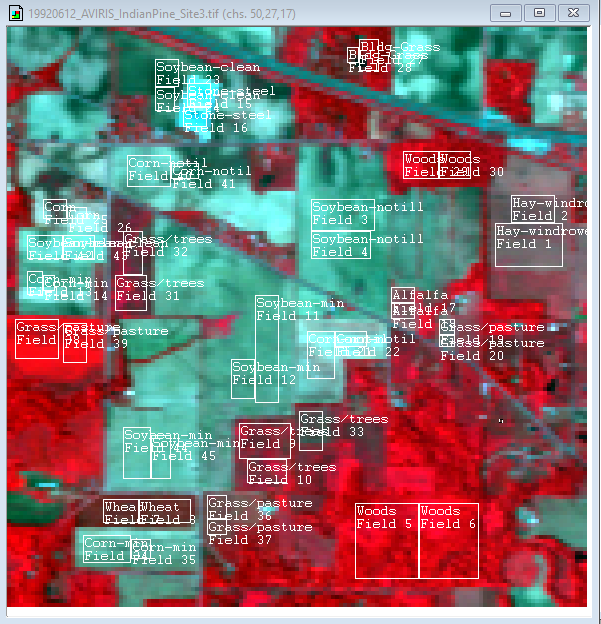
\includegraphics[height=9.0cm]{imgs/Dataset.png}
	\end{center}
	\caption{AVIRIS 92AV3C dataset for experiment}
	\label{fig:AVIRIS 92AV3C dataset for experiment}
\end{figure}

\begin{figure}[H]
	\begin{center}
		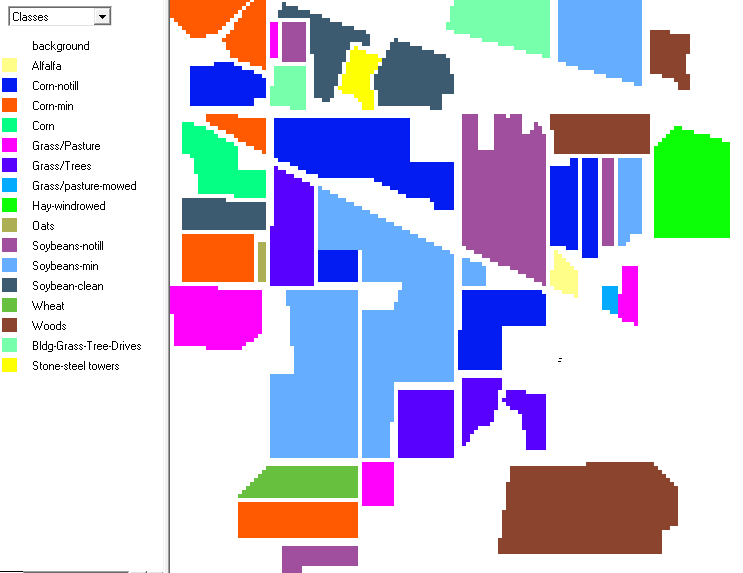
\includegraphics[height=9.0cm]{imgs/Ground.png}
	\end{center}
	\caption{Ground truth of AVIRIS 92AV3C dataset}
	\label{fig:Ground truth of AVIRIS 92AV3C dataset}
\end{figure}
\subsection{Feature Extraction Result}
\noindent In this research, at first the dimensions of the dataset is reduced from 220 using PCA. Here first few component contains most of the variation of the dataset. Figure 4.3 shows few components after applying PCA to the original AVIRIS 92AV3C dataset. First component is the most informative than second and so on. But PCA considers only the global variable of the dataset therefore some components may have more variance but less information for some specific class. Principal component 7 and principal component 9 is an example of this problem of PCA.
\begin{figure}[H]
	\begin{center}
		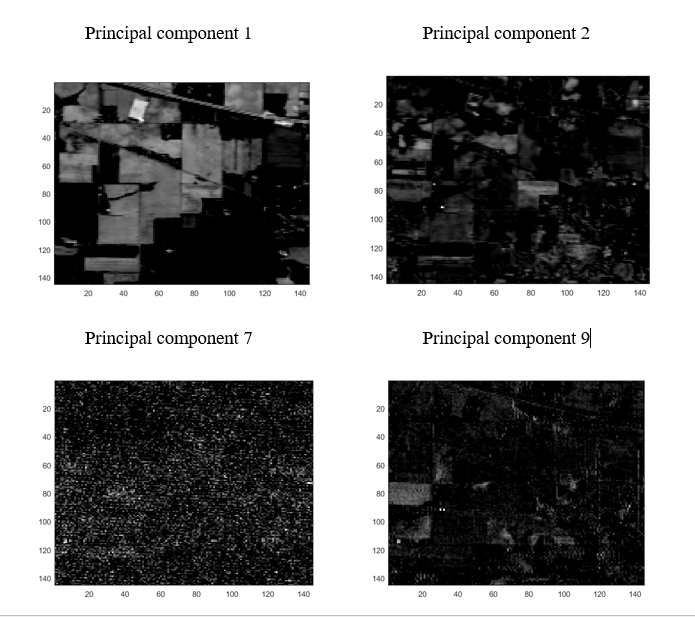
\includegraphics[height=10.0cm]{imgs/PC.png}
	\end{center}
	\caption{Some principal components}
	\label{fig:Some principal components}
\end{figure}
\begin{figure}[H]
	\begin{center}
		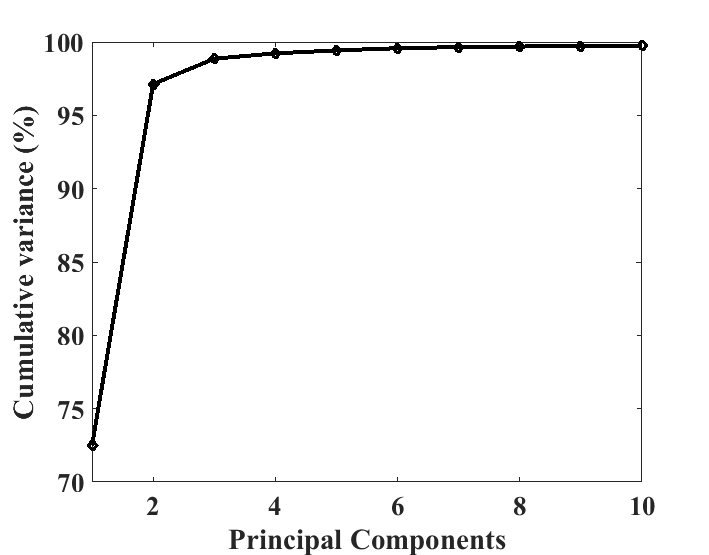
\includegraphics[height=8.0cm]{imgs/Var.png}
	\end{center}
	\caption{Cumulative variance of bands obtained via PCA}
	\label{fig:Cumulative variance of bands obtained via PCA}
\end{figure}
\noindent Figure 4.4 represents the cumulative relations between variance and each component. Here we can see than first 8 components of PCA has contain 99.69\% variations of the dataset.
\subsection{nMI Based Feature Selection Result}
\subsubsection{Original Dataset Plus nMI Approach}
\begin{table}[H]
	\caption{Selected features with Org+NMI}
	\begin{center}
		\begin{tabular}{|c|c|}
			\hline
			Method & Order of selected features\\ \hline
			Org+NMI & Band: 27,1,167,3,139,14,2,8\\ \hline
		\end{tabular}
	\end{center}
	\label{tab:Selected features with Org+NMI}
\end{table}
\begin{figure}[H]
	\begin{center}
		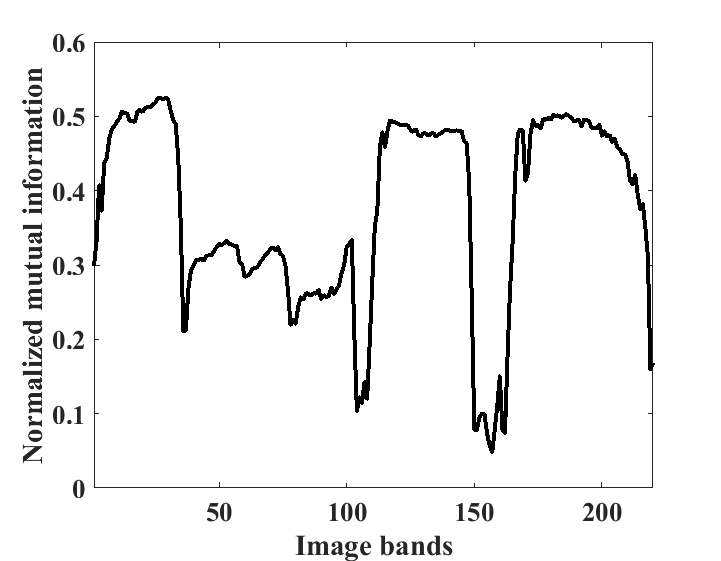
\includegraphics[height=7.0cm]{imgs/OrgNmi.png}
	\end{center}
	\caption{Normalized mutual information between class labels and original bands}
	\label{fig:Normalized mutual information between class labels and original bands}
\end{figure}
\subsubsection{PCA Dataset Plus nMI Approach}
\begin{table}[H]
	\caption{Selected features with PCA+NMI}
	\begin{center}
		\begin{tabular}{|c|c|}
			\hline
			Method & Order of selected features\\ \hline
			Org+NMI & PC: 1,4,3,5,6,9,15,2\\ \hline
		\end{tabular}
	\end{center}
	\label{tab:Selected features with PCA+NMI}
\end{table}
\begin{figure}[H]
	\begin{center}
		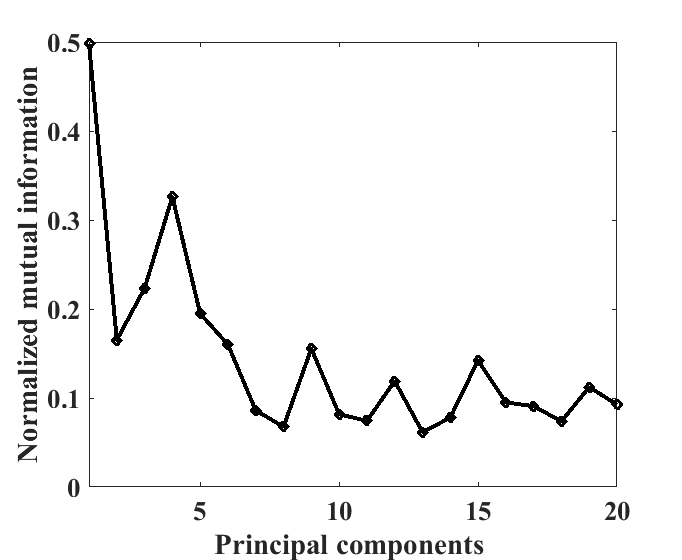
\includegraphics[height=8.0cm]{imgs/nmi.png}
	\end{center}
	\caption{Normalized mutual information between class labels and PC1-PC20}
	\label{fig:Normalized mutual information between class labels and PC1-PC20}
\end{figure}
\subsection{Proposed Method Result}
\begin{table}[H]
	\caption{Selected features for each target class with proposed method (TCO+PCA+NMI)}
	\begin{center}
		\begin{tabular}{|c|l|}
			\hline
			Target class & Order of selected features\\ \hline
			Hay-windrowed & PC: 4,1,17,5,12,3,16,2\\ \hline
			Soybean-notil & PC: 1,17,16,11,20,14,13,3\\ \hline
			Woods & PC: 1,16,17,3,15,11,5,20\\ \hline
			Wheat & PC: 6,19,17,3,12,16,11,5\\ \hline
			Grass/trees & PC: 4,9,5,6,16,17,2,1\\ \hline
			Soybean-min & PC: 1,17,16,3,5,12,11,9\\ \hline
			Corn-min & PC: 1,17,16,5,11,3,20,19\\ \hline
			Stone-steel & PC: 3,4,1,17,16,10,5,11\\ \hline
			Alfalfa & PC: 4,17,15,20,3,16,6,12\\ \hline
			Grass/Pasture & PC: 9,3,17,6,16,11,1,15\\ \hline
			Corn-notill & PC: 1,17,2,16,11,18,20,19\\ \hline
			Soybean-clean & PC: 1,15,17,3,16,20,12,11\\ \hline
			Corn & PC: 1,19,17,16,18,8,11,3\\ \hline
			Bldg-Grass & PC: 15,16,17,3,18,11,19,4\\ \hline
		\end{tabular}
	\end{center}
	\label{tab:Selected features for each target class with proposed method (TCO+PCA+NMI)}
\end{table}
\section{Classification Results}
\begin{table}[H]
	\caption{Details of the training and test samples}
	\begin{center}
		\begin{tabular}{|c|c|c|}
			\hline
			Class name & Train & Test\\ \hline
			Hay-windrowed & 187 & 77\\ \hline
			Soybean-notil & 128 & 105\\ \hline
			Woods & 367 & 341\\ \hline
			Wheat & 54 & 78\\ \hline
			Grass/trees & 249 & 115\\ \hline
			Soybean-min & 253 & 115\\ \hline
			Corn-min & 253 & 115\\ \hline
			Stone-steel & 36 & 30\\ \hline
			Alfalfa & 24 & 24\\ \hline
			Grass/Pasture & 156 & 92\\ \hline
			Corn-notill & 172 & 60\\ \hline
			Soybean-clean & 96 & 78\\ \hline
			Corn & 30 & 15\\ \hline
			Bldg-Grass & 40 & 12\\ \hline
			Total & 1900 & 1179\\ \hline
		\end{tabular}
	\end{center}
	\label{tab:Details of the training and test samples}
\end{table}

\begin{table}[H]
	\caption{Details of parameter for KSVM(RBF kernel)}
	\begin{center}
		\begin{tabular}{|c|c|c|}
			\hline
			Method & C & $\gamma$ \\ \hline
			Org+NMI & 10 & 2.44 \\ \hline
			PCA & 9 & 5.72 \\ \hline
			PCA+NMI & 10 & 6\\ \hline
			TCO+PCA+NMI & 5 & 0.75\\ \hline
		\end{tabular}
	\end{center}
	\label{tab:Details of parameter for KSVM(RBF kernel)}
\end{table}

\begin{table}[H]
	\caption{Classification result for 8 features}
	\begin{center}
		\begin{tabular}{|c|c|}
			\hline
			Method & Classification Result\\ \hline
			Org+NMI & 72.26\%\\ \hline
			PCA & 89.05\%\\ \hline
			PCA+NMI & 92.79\%\\ \hline
			TCO+PCA+NMI & 96.57\%\\ \hline
		\end{tabular}
	\end{center}
	\label{tab:Classification result for 8 features}
\end{table}

%\begin{figure}[H]
%	\begin{center}
%		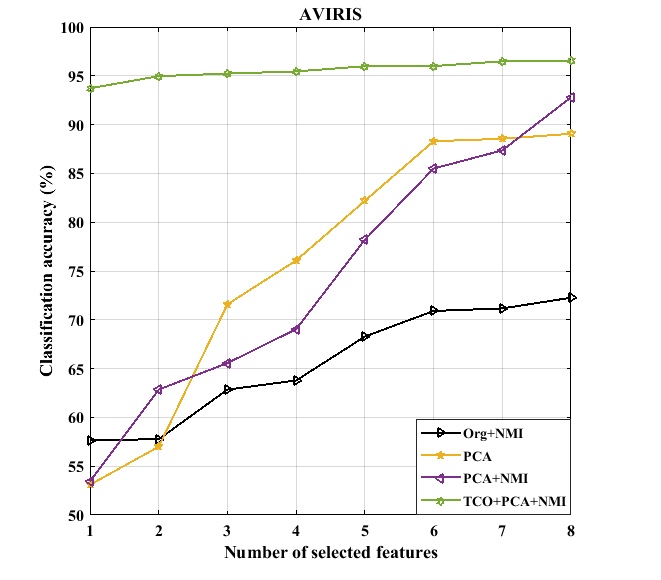
\includegraphics[height=10.0cm]{imgs/4MethodsAc.png}
%	\end{center}
%	\caption{Classification accuracy of AVIRIS 92AV3c data}
%	\label{fig:Classification accuracy of AVIRIS 92AV3c data}
%\end{figure}

\end{document}